
%(BEGIN_QUESTION)
% Copyright 2012, Tony R. Kuphaldt, released under the Creative Commons Attribution License (v 1.0)
% This means you may do almost anything with this work of mine, so long as you give me proper credit

Sketch connecting wires so that this DAQ unit will register an increasing positive measurement on channel 4 as the potentiometer shaft is turned {\it counter-clockwise}:

$$\includegraphics[width=15.5cm]{i02125x01.eps}$$

\vskip 20pt \vbox{\hrule \hbox{\strut \vrule{} {\bf Suggestions for Socratic discussion} \vrule} \hrule}

\begin{itemize}
\item{} An important determination for any DAQ unit is whether its inputs are {\it single-ended} or {\it differential}.  How can we tell, in this instance?
\item{} Re-sketch the circuit to yield an increasing positive measurement on channel 4 as the potentiometer shaft is turned {\it clockwise}.
\end{itemize}

\underbar{file i02125}
%(END_QUESTION)





%(BEGIN_ANSWER)


%(END_ANSWER)





%(BEGIN_NOTES)

$$\includegraphics[width=15.5cm]{i02125x02.eps}$$

%INDEX% Pictorial circuit review (analog signal wiring to data acquisition unit)

%(END_NOTES)


